% Model 1 "two clocks": inner day dial (water bucket, one turn = one year),
% outer year ring (cover, one step per turn). They meet only at 12 o'clock (year end).
% Build: cd Paper/Figure && pdflatex m1_two_clocks.tex
\documentclass[tikz,border=3pt]{standalone}
\usepackage{newtxtext,newtxmath}
\usepackage{amsmath}
\usetikzlibrary{arrows.meta,calc}
\definecolor{yr}{HTML}{18473C}      % year clock (dark green)
\definecolor{yrBg}{HTML}{E3F4EE}
\definecolor{dy}{HTML}{2B6CB0}      % day clock (water blue)
\definecolor{dyBg}{HTML}{E6F0FA}
\definecolor{gs}{HTML}{F3D9A4}      % growing season
\tikzset{badge/.style={circle, draw=#1, fill=white, line width=0.8pt, inner sep=0.5pt,
  font=\scriptsize\bfseries, text=#1, minimum size=10pt, solid}}
\begin{document}
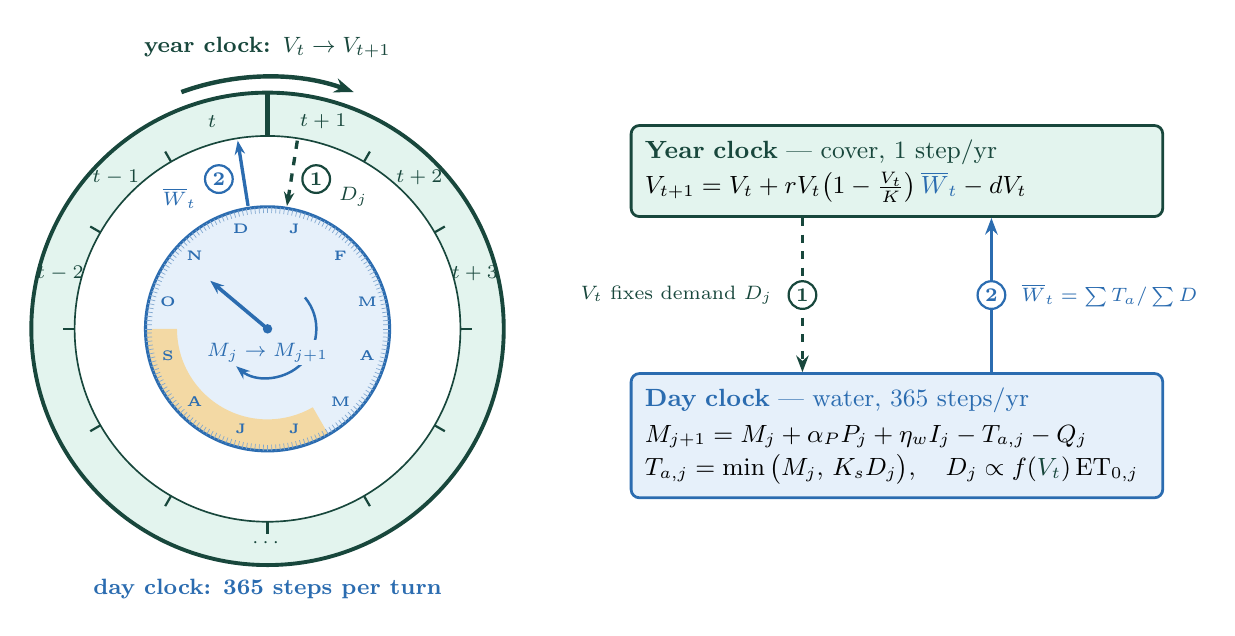
\begin{tikzpicture}[font=\small]
\def\Ro{3.0}\def\Rm{2.45}\def\Ri{1.55}
% ---------- outer ring: year clock (one sector = one year) ----------
\fill[yrBg] (0,0) circle (\Ro);
\fill[white] (0,0) circle (\Rm);
\draw[yr, line width=1.4pt] (0,0) circle (\Ro);
\draw[yr, line width=0.6pt] (0,0) circle (\Rm);
\foreach \a in {0,30,...,330} \draw[yr, line width=0.8pt] (\a:\Rm) -- (\a:\Rm+0.15);
\foreach \a/\l in {165/{t-2},135/{t-1},105/{t},75/{t+1},45/{t+2},15/{t+3}}
  \node[yr, font=\scriptsize] at (\a:{(\Ro+\Rm)/2}) {$\l$};
\node[yr, font=\scriptsize] at (-90:{(\Ro+\Rm)/2}) {$\cdots$};
\draw[yr, line width=2pt] (90:\Rm) -- (90:\Ro);                 % year boundary
\draw[yr, line width=1.6pt, -{Stealth[length=7pt]}] (110:\Ro+0.2) arc (110:70:\Ro+0.2);
\node[yr, font=\footnotesize\bfseries, above] at (0,\Ro+0.32) {year clock: $V_t\to V_{t+1}$};

% ---------- inner dial: day clock (one turn = one year) ----------
\fill[dyBg] (0,0) circle (\Ri);
\fill[gs] (90-30*5:\Ri) arc (90-30*5:90-30*9:\Ri) -- (90-30*9:\Ri-0.4) arc (90-30*9:90-30*5:\Ri-0.4) -- cycle;
\draw[dy, line width=1.1pt] (0,0) circle (\Ri);
\foreach \a in {0,2,...,358} \draw[dy!60, line width=0.25pt] (\a:\Ri) -- (\a:\Ri-0.08);
\foreach \m/\l in {1/J,2/F,3/M,4/A,5/M,6/J,7/J,8/A,9/S,10/O,11/N,12/D}
  \node[dy, font=\tiny\bfseries] at (90-30*\m+15:\Ri-0.24) {\l};
\draw[dy, line width=1.3pt, -{Stealth[length=5pt]}] (0,0) -- (140:0.95);   % fast hand
\fill[dy] (0,0) circle (0.06);
\draw[dy, line width=0.9pt, -{Stealth[length=5pt]}] (40:0.62) arc (40:-130:0.62);
\node[dy, font=\scriptsize, fill=dyBg, inner sep=1pt] at (0,-0.3) {$M_j\to M_{j+1}$};
\node[dy, font=\footnotesize\bfseries, below] at (0,-\Ro-0.05) {day clock: 365 steps per turn};

% ---------- the two handoffs, both at the year boundary ----------
\draw[dy, line width=1.2pt, -{Stealth[length=5pt]}] (99:\Ri+0.03) -- (99:\Rm-0.03);
\draw[yr, line width=1.2pt, dashed, -{Stealth[length=5pt]}] (81:\Rm-0.03) -- (81:\Ri+0.03);
\node[badge=dy] at (108:{(\Ri+\Rm)/2}) {2};
\node[dy, font=\scriptsize] at (124:{(\Ri+\Rm)/2}) {$\overline W_t$};
\node[badge=yr] at (72:{(\Ri+\Rm)/2}) {1};
\node[yr, font=\scriptsize] at (57:{(\Ri+\Rm)/2}) {$D_j$};

% ---------- equation panel ----------
\begin{scope}[xshift=4.6cm]
\node[draw=yr, line width=1pt, fill=yrBg, rounded corners=3pt, text width=6.4cm, align=left, inner sep=5pt, anchor=north west] (Y) at (0,2.6) {%
  {\color{yr}\textbf{Year clock} --- cover, 1 step/yr}\\[2pt]
  $V_{t+1}=V_t+rV_t\big(1-\tfrac{V_t}{K}\big)\,{\color{dy}\overline W_t}-dV_t$};
\node[draw=dy, line width=1pt, fill=dyBg, rounded corners=3pt, text width=6.4cm, align=left, inner sep=5pt, anchor=north west] (D) at (0,-0.55) {%
  {\color{dy}\textbf{Day clock} --- water, 365 steps/yr}\\[2pt]
  $M_{j+1}=M_j+\alpha_PP_j+\eta_wI_j-T_{a,j}-Q_j$\\[1pt]
  $T_{a,j}=\min\big(M_j,\,K_s D_j\big),\quad D_j\propto f({\color{yr}V_t})\,\mathrm{ET}_{0,j}$};
\draw[yr, line width=1pt, dashed, -{Stealth[length=6pt]}] ([xshift=-1.2cm]Y.south) -- node[badge=yr, pos=0.5] (b1) {1} ([xshift=-1.2cm]D.north);
\node[yr, font=\scriptsize, left=2pt] at (b1.west) {$V_t$ fixes demand $D_j$};
\draw[dy, line width=1pt, -{Stealth[length=6pt]}] ([xshift=1.2cm]D.north) -- node[badge=dy, pos=0.5] (b2) {2} ([xshift=1.2cm]Y.south);
\node[dy, font=\scriptsize, right=2pt] at (b2.east) {$\overline W_t=\sum T_a/\sum D$};
\end{scope}
\end{tikzpicture}
\end{document}
